	\documentclass[10pt,]{article}
\usepackage{../style}
\begin{document}
\begin{listofex}
	\item Треугольник \( ABC \) --- равнобедренный (\( AB=BC \)), \( \angle B=120\degree \). Найдите площадь треугольника \( ABC \), если высота \( BH=\dfrac{\sqrt{3}}{2} \).
	\begin{center}
		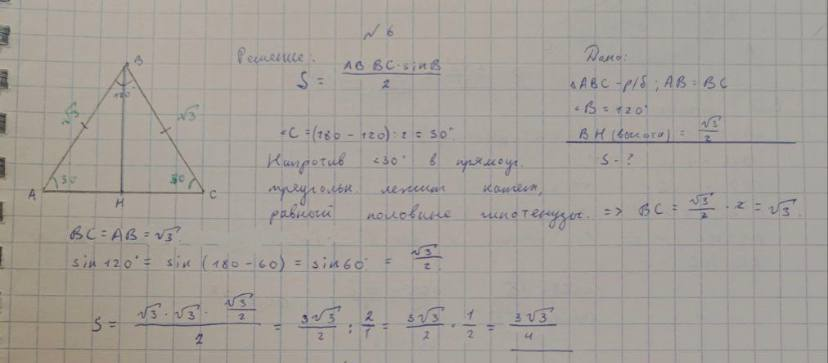
\includegraphics[align=t, width=1\linewidth]{../exercises/lists/pics/curator1}
	\end{center}
	\item Решите неравенство: \(|4x^2+5x-6|\le0\)
	\begin{center}
		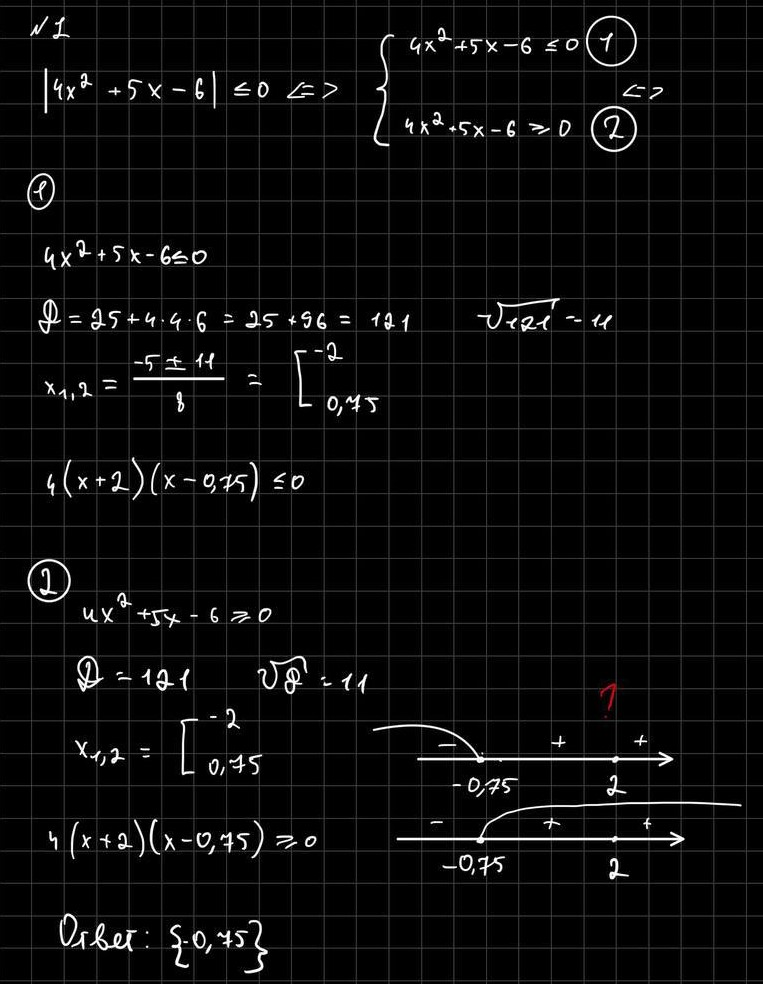
\includegraphics[align=t, width=0.55\linewidth]{../exercises/lists/pics/curator2}
	\end{center}
\newpage
	\item Решите неравенство: \(\dfrac{x^3-4x^2-25x+100}{4-x}\ge0\)
	\begin{center}
		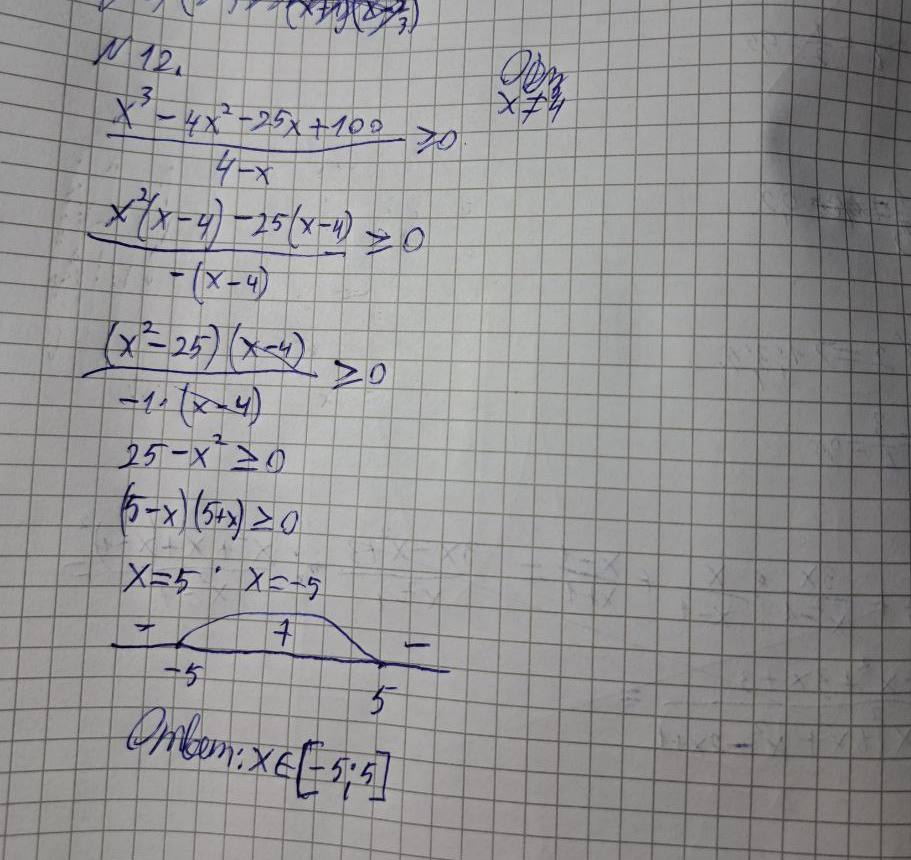
\includegraphics[align=t, width=1\linewidth]{../exercises/lists/pics/curator3}
	\end{center}
\newpage
	\item Окружность построена на стороне \( AB \) треугольника \( ABC \) как на диаметре и пересекает сторону \( AC \) в точке \( K \). Докажите, что треугольник \( ABC \) равнобедренный, если \( AK=KC \).
	 \begin{center}
	 	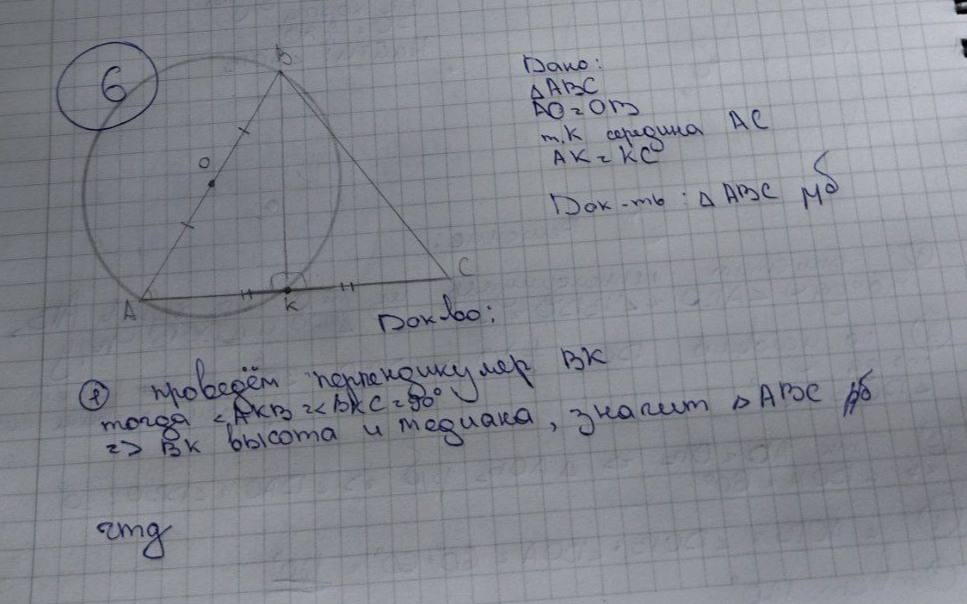
\includegraphics[align=t, width=1\linewidth]{../exercises/lists/pics/curator4}
	 \end{center}
 \newpage
 	\item Определите, при каких значениях \( m \) вершины парабол \( y=x^2+4mx+2 \) и \( y=-x^2+2mx+4 \) будут находиться по одну сторону от оси \( x \).
 	\begin{center}
 		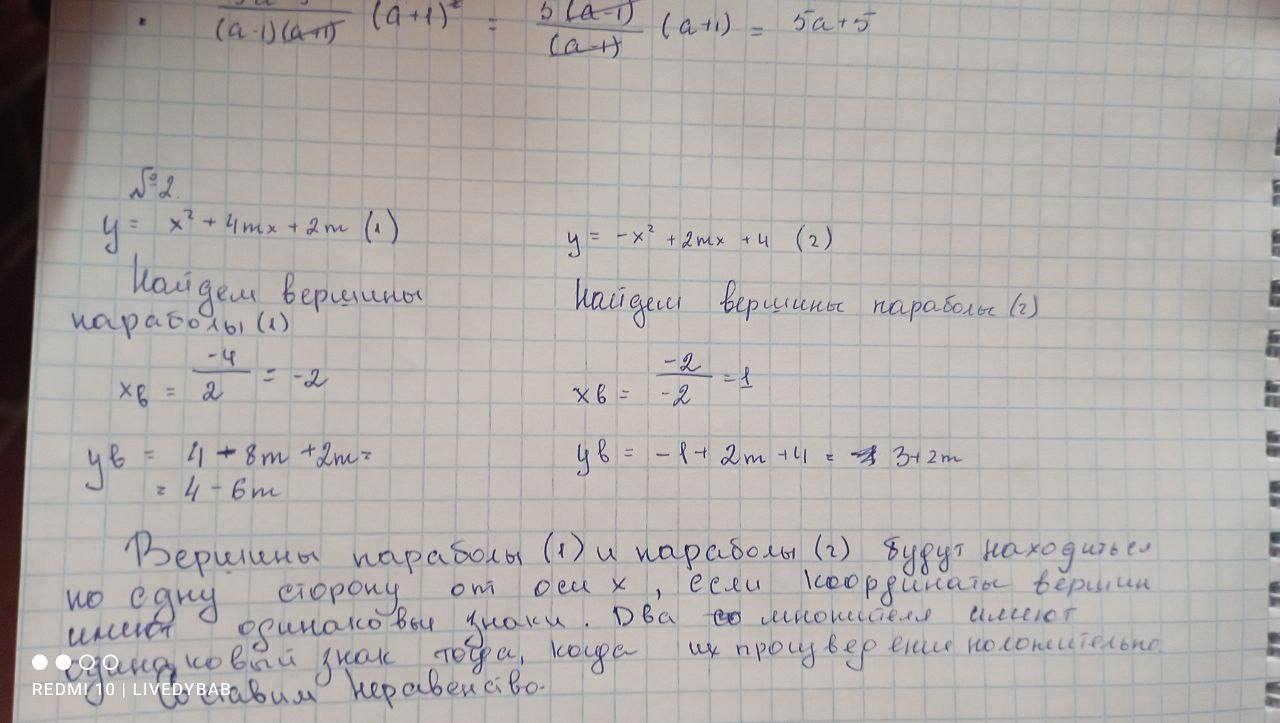
\includegraphics[align=t, width=1\linewidth]{../exercises/lists/pics/curator5}
 	\end{center}
	 \begin{center}
	 	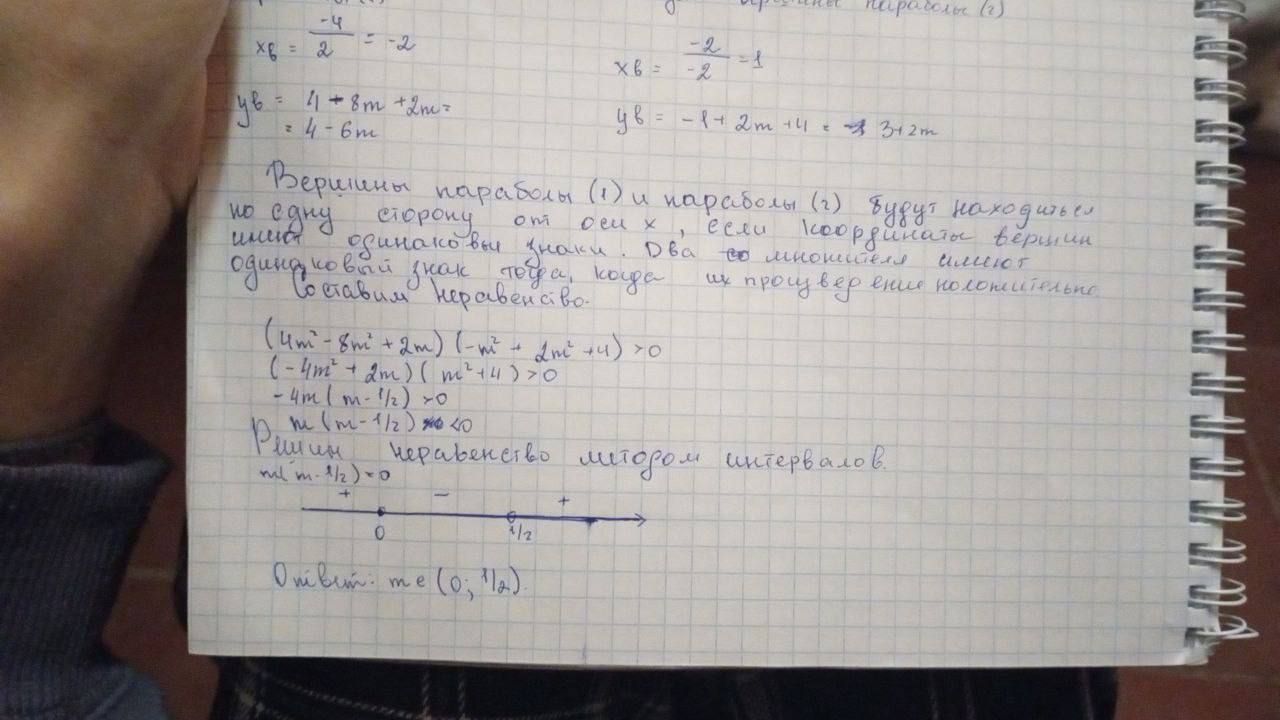
\includegraphics[align=t, width=1\linewidth]{../exercises/lists/pics/curator6}
	 \end{center}
 \newpage
 	\item Решите уравнение: \((x+8)\log_{x+4}(x+1)=0\)
 	\begin{center}
 		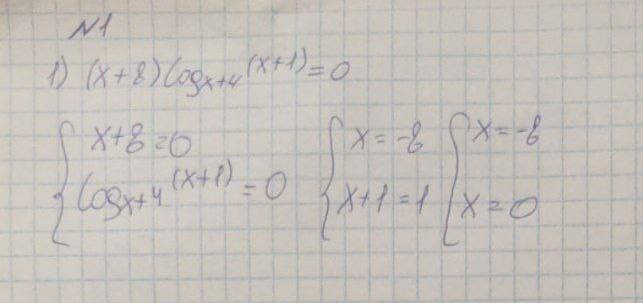
\includegraphics[align=t, width=1\linewidth]{../exercises/lists/pics/curator7}
 	\end{center}
 	\item Решите уравнение: \(|x^2-2x-3|=3-x\)
	\item На катетах \( AC \) и \( BC \) прямоугольного треугольника \( ABC \) вне его построены квадраты \( ACDE \) и \( CBFK \) (вершины обоих квадратов перечислены против часовой стрелки)., \( P \) --- середина \( KD \). Докажите, что \( CP\perp AB \).
 	\item Дана окружность с центром \( O \). На продолжении хорды \( AB \) за точку \( B \) отложен отрезок \( BC \), равный радиусу. Через точки \( C \) и \( O \) проведена секущая \( CD \) (\( D \) --- точка пересечения с окружностью, лежащая вне отрезка \( CO \)). Докажите, что \( \angle AOD=3\angle ACD \).
 	\item Первый насос наполняет бак за \( 20 \) минут, второй --- за \( 30 \) минут, а третий --- за \( 1 \) час. За сколько минут наполнят бак три насоса, работая одновременно? 
	\item Сколько существует чётных пятизначных чисел?
	\item Докажите, что число \( 10^{2011}+2015 \) делится на \( 9 \).
\end{listofex}
\end{document}